\documentclass[a4paper,12pt]{report}
\usepackage[T2A]{fontenc}
\usepackage[utf8]{inputenc}
\usepackage[english,russian]{babel}
\usepackage{graphicx}
\usepackage{wrapfig}
\usepackage{mathtext} 				% русские буквы в фомулах
\usepackage{amsmath,amsfonts,amssymb,amsthm,mathtools} % AMS
\usepackage{icomma} % "Умная" запятая: $0,2$ --- число, $0, 2$ --- перечисление
\usepackage{capt-of}
\usepackage{appendix}
\usepackage{multirow}
\usepackage{hyperref}
\usepackage{floatrow}
\usepackage[left=2cm,right=2cm,
    top=2cm,bottom=2cm,bindingoffset=0cm]{geometry}
\usepackage{multicol} % Несколько колонок
\usepackage{gensymb}
\title{Отчёт по лабораторной работе №5

Генераторы синусоидальных колебаний с кварцевой стабилизацией}
\author{Плюскова Н.А. Б04-004 }
\date{\today}

\begin{document}

\maketitle

\section*{1. Результаты эксперимента}
\subsection*{1.1 Резонансный усилитель}

Соберем схему, показанную на рис.\ref{p1}:

\begin{figure}[H]
    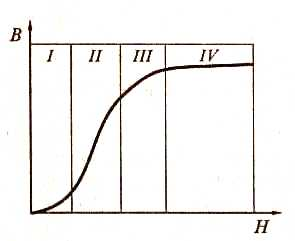
\includegraphics[scale=0.2]{pic1.jpg}
    \caption{Схема резонансного усилителя}
    \label{p1}
\end{figure}


Напряжения $U_{out_1}$, $U_{out}$ связаны теоретическим соотношением:
    \[ \beta_{теор}= \frac{U_{out_1}}{U_{out}} = \frac{C_3}{C_3 + C_4} \approx \frac{1}{7} \]

При проведении эксперимента получили значения $U_{out_1} \approx 201 \text{ мВ}$, $U_{out} \approx 1638 \text{ мВ}$. Таким образом, практическое значение несильно отличается:

    \[ \beta_{практ}= \frac{U_{out_1}}{U_{out}} \approx \frac{1}{8} \]

С помощью конденсатора с переменной емкостью добиваемся частоты колебаний $f_p = 1 \text{ МГц}$. 

На резонансной частоте $f_p$ снимем амплитудную характеристику усилителя (см. рис.\ref{p2}):

\begin{table}[H]
\begin{tabular}{|c|c|}
\hline
$U_{in}$, мВ & $K$    \\ \hline
10        & 4,96 \\ \hline
20        & 4,91 \\ \hline
30        & 4,92 \\ \hline
40        & 4,92 \\ \hline
50        & 4,93 \\ \hline
60        & 4,95 \\ \hline
70        & 4,95 \\ \hline
80        & 5,02 \\ \hline
90        & 5,03 \\ \hline
100       & 5,04 \\ \hline
200       & 4,95 \\ \hline
300       & 4,55 \\ \hline
400       & 3,81 \\ \hline
500       & 3,18 \\ \hline
\end{tabular}
\caption{Амплитудная характеристика усилителя}
\end{table}

\begin{figure}[H]
    \includegraphics[scale=0.7]{K(U_out).png}
    \caption{Амплитудная характеристика усилителя}
    \label{p2}
\end{figure}

Соединив накоротко эмиттеры транзисторов, измерим резонансный коэффициент усиления: $K = 3,5$

Снимем зависимость коэффициента усиления от частоты входного сигнала при амплитуде $U_{in} = 80$ мВ (см. рис.\ref{p3}):

\begin{table}[H]
\begin{tabular}{|c|c|}
\hline
$f$,МГц & $K$     \\ \hline
1,00  & 10,11 \\ \hline
1,60  & 0,71  \\ \hline
1,30  & 1,34  \\ \hline
1,10  & 4,37  \\ \hline
1,20  & 1,96  \\ \hline
1,06  & 7,31  \\ \hline
1,07  & 6,07  \\ \hline
1,05  & 8,98  \\ \hline
0,98  & 6,73  \\ \hline
0,99  & 8,18  \\ \hline
\end{tabular}
\caption{Зависимость коэффициента усиления от частоты входного сигнала}
\end{table}

\begin{figure}[H]
    \includegraphics[scale=0.7]{K(f).png}
    \caption{Зависимость $K(f)$}
    \label{p3}
\end{figure}

Получим, что $\Delta f_{0,7} \approx 80$ кГц. Откуда получим добротность: $Q = \frac{f_{p}}{\Delta f_{0,7}} = 12,5$

\subsection*{1.2 Кварцевый генератор с использованием последовательного резонанса кварца}

Соберем схему, изображенную на рис.\ref{p4}:

\begin{figure}[H]
    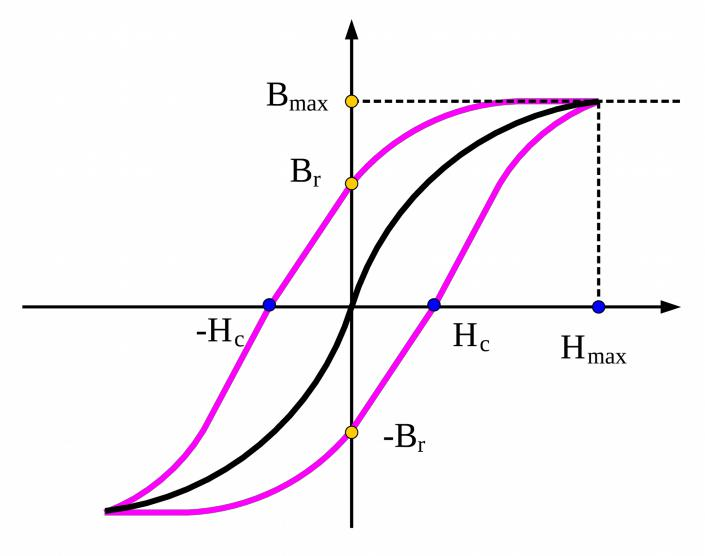
\includegraphics[scale=0.2]{pic2.jpg}
    \caption{Схема установки кварцевого генератора}
    \label{p4}
\end{figure}

Измерим амплитуду выходного колебания $U_{out} = 7,36$ В, что сходится с ожидаемым значением $U_{out} = 7,25$ В

Восстановим схему кварцевого генератора, включив между эмиттерами кварцевый резонатор вместо резистора R.

После расстройки LC-контура путем добавления конденсатора $\Delta C = 15$ пФ измерим изменения частоты колебаний $\Delta f$ без кварца и $\Delta f_{\text{к}}$ с кварцем:
\begin{equation*}
    \Delta f = 3 \text{ Гц}
\end{equation*}
\begin{equation*}
    \Delta f_{\text{к}} = 16554 \text{ Гц}
\end{equation*}

Откуда из соотношения $\frac{\Delta f_{\text{к}}}{\Delta f} = \frac{Q}{Q_{\text{к}}}$ находим $Q_{\text{к}} = 9 \cdot 10^{5}$

Восстановим настройку контура в резонанс. Для этого включим последовательно конденсатор $C_{s} = 121$ пФ. Получим $\Delta f_{\text{к}} = 25$ Гц. Из формулы $\frac{\Delta f_{\text{к}}}{\Delta f} = \frac{C_{\text{к}}}{2C_{s}}$ определим $C_{\text{к}} = 6\cdot 10^{-15}$ пФ. Остальные параметры найдем расчетным путем:
\begin{equation*}
    L_{\text{к}} = \frac{1}{4\pi^2 f_{\text{к}}^2 C_{\text{к}}} = 4,19 \text{Гн}
\end{equation*}
\begin{equation*}
    \rho_{\text{к}} = \sqrt{\frac{L_{\text{к}}}{C_{\text{к}}}} = 2\pi f_{\text{к}} L_{\text{к}} = \frac{1}{2\pi f_{\text{к}} C_{\text{к}}} = 2,65 \cdot 10^7 \text{МОм}
\end{equation*}
\begin{equation*}
    r_{\text{к}} = \frac{\rho_{\text{к}}}{Q_{\text{к}}} = 29,4 \text{Ом}
\end{equation*}

Снимем зависимость частоты генерируемых колебаний от напряжения $U_{\text{п}_2}$:

\begin{table}[H]
\begin{tabular}{|c|c|}
\hline
$U_{\text{п}_2}$, В & $f$, МГц   \\ \hline
8        & 1,001540 \\ \hline
9        & 1,000935 \\ \hline
10       & 1,000435 \\ \hline
11       & 0,999763 \\ \hline
12       & 0,998848 \\ \hline
\end{tabular}
\caption{Зависимость частоты генерируемых колебаний с кварцем от входного напряжения}
\end{table}

Снимем аналогичную зависимость для генератора без кварца:

\begin{table}[H]
\begin{tabular}{|c|c|}
\hline
$U_{\text{п}_2}$, В & $f$, МГц  \\ \hline
8        & 1,00044 \\ \hline
9        & 1,00041 \\ \hline
10       & 1,00004 \\ \hline
11       & 1,00038 \\ \hline
12       & 1,00035 \\ \hline
\end{tabular}
\caption{Зависимость частоты генерируемых колебаний без кварца от входного напряжения}
\end{table}

\end{document}
